\chapter{Proofs and complements of Chapter~\ref{chap:Timelines}}
\minitoc\mtcskip


\section{Definition of the value transition function $T$ in the proof of Theorem~\ref{theorem:undecidability}}\label{sec:undecidabilityTrans}

The value transition function $T$ of $x_M$ is defined as follows.
 \begin{itemize}
   \item For each instruction label $\ell\in \Inc \cup \{\ell_\halt\}$, let $P_\ell=\emptyset$ if $\ell=\ell_\halt$,
   and $P_\ell=\{(\Succ(\ell),\inc_h)\}$ otherwise, where $c_h= c(\ell)$. Then, $T(\ell)$, $T((\ell,c_i))$, and $T((\ell,(c_i,\#))$, for $i=1,2$, are defined as follows:
   %
\[
T(\ell)   =  \{(\ell,c_1),(\ell,c_2)\}\cup P_\ell 
\]

\[
T((\ell,c_1))   =  \{(\ell,c_1),(\ell,c_2)\}\cup P_\ell
\]

\[
T((\ell,c_2))   =  \{(\ell,c_2)\}\cup P_\ell % \\
\]
%
\item For each  instruction label $\ell\in\Dec$ and for each $\ell'\in \{\zero(\ell),\dec(\ell)\}$, $T((\ell,\ell'))$, $T((\ell,\ell',c_i))$, and $T((\ell,\ell',(c_i,\#))$, for $i=1,2$, are defined as:
%
 \[
    T((\ell,\ell'))  =  \left\{
      \begin{array}{ll}
        \{(\ell,\ell',c_2),(\ell',\zero_1)\}
        &    \text{if }  c(\ell) =c_1 , \ell'=\zero(\ell)
        \\
        \{(\ell,\ell',c_1),(\ell',\zero_2)\}
        &    \text{if }  c(\ell) =c_2 , \ell'=\zero(\ell)
        \\
        \{(\ell,\ell',(c_1,\#))\}
        &    \text{if }  c(\ell) =c_1 , \ell'=\dec(\ell)
        \\
        \{(\ell,\ell', c_1),(\ell,\ell',(c_2,\#))\}
        &    \text{otherwise }
       \end{array}
    \right.
  \]
 %
  \[
    T((\ell,\ell',c_1))  =  \left\{
      \begin{array}{ll}
        \emptyset
        &    \text{if }  c(\ell)\! =\!c_1 , \ell'\!=\!\zero(\ell)
        \\
        \{(\ell,\ell',c_1),(\ell',\zero_2)\}
        &    \text{if }  c(\ell)\! =\!c_2 , \ell'\!=\!\zero(\ell)
        \\
        \{(\ell,\ell',c_1),(\ell,\ell',c_2),(\ell',\dec_1)\}
        &    \text{if }  c(\ell)\! =\!c_1 , \ell'\!=\!\dec(\ell)
        \\
        \{(\ell,\ell', c_1),(\ell,\ell',(c_2,\#))\}
        &    \text{otherwise }
       \end{array}
    \right.
  \]
 %
  \[
    T((\ell,\ell',c_2))  =  \left\{
      \begin{array}{ll}
      \{(\ell,\ell',c_2),(\ell',\zero_1)\}
        &    \text{if }  c(\ell) =c_1 , \ell'=\zero(\ell)
        \\
       \emptyset
        &    \text{if }  c(\ell) =c_2 , \ell'=\zero(\ell)
        \\
        \{ (\ell,\ell',c_2),(\ell',\dec_1)\}
        &    \text{if }  c(\ell) =c_1 , \ell'=\dec(\ell)
        \\
        \{ (\ell,\ell',c_2),(\ell',\dec_2)\}
        &    \text{otherwise }
       \end{array}
    \right.
  \]
 %
   \[
    T((\ell,\ell',(c_1,\#)))  =  \left\{
      \begin{array}{ll}
        \{(\ell,\ell'\!,c_1),\!(\ell,\ell'\!,c_2),\!(\ell'\!,\dec_1)\}
        &    \text{if }  c(\ell) \!=\! c_1 , \ell'\!\!=\!\dec(\ell)
        \\
         \emptyset
        &    \text{otherwise }
       \end{array}
    \right.
  \]
 %
   \[
    T((\ell,\ell',(c_2,\#)))  =  \left\{
      \begin{array}{ll}
        \{ (\ell,\ell',c_2),(\ell',\dec_2)\}
        &    \text{if }  c(\ell) = c_2 , \ell'=\dec(\ell)
        \\
         \emptyset
        &    \text{otherwise }
       \end{array}
    \right.
  \]


 \item For each label $\ell\in\InstructLab$ and operation $\op\in\{\inc_1,\inc_2,\zero_1,\zero_2,\dec_1,\allowbreak \dec_2\}$, $T((\ell,\op))$, $T((\ell,\op,c_i))$, and $T((\ell,\op,(c_i,\#))$, for $i=1,2$, are defined as follows,
 where $S_\ell=\{(\ell,\zero(\ell)),(\ell,\dec(\ell))\}$ if $\ell\in\Dec$, and $S_\ell=\{\ell\}$ otherwise:
\[
    T((\ell,\op))  =  \left\{
      \begin{array}{ll}
        \{(\ell,\op,c_2)\}\cup S_\ell
        &    \text{if }  \op = \zero_1 , \ell\neq \ell_\init
        \\
        \{(\ell,\op,c_1)\} \cup S_\ell
        &    \text{if }  \op = \zero_2 , \ell\neq \ell_\init
        \\
        \{(\ell,\op,c_1),(\ell,\op,c_2)\} \cup S_\ell
        &    \text{if }  \op \in \{\dec_1,\dec_2\} , \ell\neq \ell_\init
        \\
        \{(\ell,\op,(c_1,\#))\}
        &    \text{if }  \op = \inc_1 , \ell\neq \ell_\init
        \\
        \{(\ell,\op,c_1),(\ell,\op,(c_2,\#))\}
        &    \text{if }  \op = \inc_2 , \ell\neq \ell_\init\\
        \{\ell_\init\}  &    \text{if }  \op = \zero_1 , \ell= \ell_\init\\
         \emptyset
        &    \text{otherwise}
      \end{array}
    \right.
  \]
 %
\[
    T((\ell,\op,c_1))  =  \left\{
      \begin{array}{ll}
        \emptyset
        &    \text{if }   \op = \zero_1 \text{ or } \ell =\ell_\init
        \\
        \{(\ell,\op,c_1)\} \cup S_\ell
        &    \text{if }  \op = \zero_2 , \ell\neq \ell_\init
        \\
        \{(\ell,\op,c_1),(\ell,\op,c_2)\} \cup S_\ell
        &    \text{if }  \op \in \{\dec_1,\dec_2,\inc_1\} , \\ & \phantom{if }\ell\neq \ell_\init
        \\
         \{(\ell,\op,c_1),(\ell,\op,(c_2,\#))\}
        &    \text{if }  \op = \inc_2 , \ell\neq \ell_\init
      \end{array}
    \right.
  \]
%
\[
    T((\ell,\op,c_2))  =  \left\{
      \begin{array}{ll}
        \emptyset
        &    \text{if }   \op = \zero_2 \text{ or } \ell =\ell_\init
        \\
         \{(\ell,\op,c_2)\} \cup S_\ell
        &    \text{otherwise }
      \end{array}
    \right.
  \]
  %
  \[
    T((\ell,\op,(c_1,\#)))  =  \left\{
      \begin{array}{ll}
        \emptyset
        &    \text{if }   \op \neq \inc_1 \text{ or } \ell =\ell_\init
        \\
        \{(\ell,\op,c_1),(\ell,\op,c_2)\} \cup S_\ell
        & \text{otherwise }
      \end{array}
    \right.
  \]
  %
  \[
    T((\ell,\op,(c_2,\#)))  =  \left\{
      \begin{array}{ll}
        \emptyset
        &    \text{if }   \op \neq \inc_2 \text{ or } \ell =\ell_\init
        \\
        \{(\ell,\op,c_2)\} \cup S_\ell
        & \text{otherwise }
      \end{array}
    \right.
  \]
  \end{itemize}

This concludes the definition of $T$ of $x_M$.

\section{Non-primitive recursive-hardness of future \allowbreak TP}\label{sec:NPRHardness}

In this section, we establish the following result.
\begin{theorem*}[\ref{theorem:NPRHardness}]
The future TP problem, even with \emph{one state variable}, is non-primitive recursive-hard also under one of the following two assumptions: \emph{either} $(1)$~the trigger rules are simple,
\emph{or} $(2)$~the intervals are in $\Intv_{(0,\infty)}$. %
%\footnote{We refer to intervals in rules' atoms and in the constraint functions of state variables.}.
\end{theorem*}

Theorem~\ref{theorem:NPRHardness} is proved by a polynomial-time reduction from the halting problem for \emph{gainy counter machines}~\cite{DemriL09}, a variant of standard Minsky machines, whose counters may erroneously  increase. Such a machine is a tuple $M = \tpl{Q,q_\init,q_\halt,n, \Delta}$,
where:
%
\begin{itemize}
  \item  $Q$ is a finite set of (control) locations/states, $q_\init\in Q$ is the initial location, and $q_\halt\in Q$ is the halting location,
  \item  $n\in\Nat\setminus\{0\}$ is the number of counters of $M$, and
  \item $\Delta \subseteq Q\times \InstL \times Q$ is a transition relation over the instruction set $\InstL= \{\inc,\dec,\allowbreak \zero\}\times \{1,\ldots,n\}$.
\end{itemize}%\vspace{0.1cm}
%
We adopt the following notational conventions.
 For an instruction
$\instr\in \InstL$, let $c(\instr)\in\{1,\ldots,n\}$ be the counter associated with $\instr$.
For a transition $\delta\in \Delta$ of the form $\delta=(q,\instr,q')$, we define $\From(\delta)= q$, $\instr(\delta)=\instr$, $c(\delta)= c(\instr)$,
and $\To(\delta)= q'$.  We denote by $\instr_\init$ the instruction $(\zero,1)$.
%
W.l.o.g., we make these assumptions:
\begin{itemize}
  \item for each transition $\delta\in \Delta$, $\From(\delta)\neq q_\halt$ and $\To(\delta )\neq q_\init$, and
    \item there is exactly one transition in $\Delta$, denoted $\delta_\init$, having as source the initial location $q_\init$.
\end{itemize}%\vspace{0.2cm}

An \emph{$M$-configuration} is a pair $(q,\nu)$ consisting of a location $q\in Q$ and a counter valuation $\nu: \{1,\ldots,n\}\to \Nat$. Given
two valuations $\nu$ and $\nu'$, we write $\nu\geq \nu'$ if and only if $\nu(c)\geq \nu'(c)$ for all $c\in\{1,\ldots,n\}$.


Under the \emph{exact semantics} (with no errors), $M$ induces a transition relation, denoted by $\longrightarrow$, over pairs of $M$-configurations and instructions, defined as follows:
 for configurations $(q,\nu)$ and $(q',\nu')$, and instructions $\instr \in \InstL$, we have $(q,\nu) \der{\instr} (q',\nu')$ if the following holds, where $c\in \{1,\ldots,n\}$ is the counter associated with the instruction
 $\instr$:
 %
\begin{itemize}
  \item  $(q,\instr,q')\in \Delta$ and $\nu'(c')= \nu(c')$ for all $c'\in \{1,\ldots,n\}\setminus\{c\}$;
  \item  $\nu'(c)= \nu(c) +1$ if $\instr=(\inc,c)$;
  \item $\nu'(c)= \nu(c) -1$ if $\instr=(\dec,c)$ (in particular, it has to be $v(c)>0$);
   \item  $\nu'(c)= \nu(c)=0$ if $\instr=(\zero,c)$.
\end{itemize}%\vspace{0.1cm}

%

The \emph{gainy semantics} is obtained from the exact one by allowing \emph{increment} errors.
Formally, %under the gainy semantics,
$M$  induces a transition relation, denoted by $\longrightarrow_\gainy$, defined as follows:
for configurations $(q,\nu)$ and $(q',\nu')$, and instructions $\instr \in \InstL$, we have $(q,\nu) \derG{\instr} (q',\nu')$ if the following holds, where $c=c(\instr)$ is the counter associated with the instruction
$\instr$:
$(q,\nu) \derG{\instr} (q',\nu')$ iff there are valuations $\nu_+$ and $\nu'_+$ such that
$\nu_+ \geq \nu$, $(q,\nu_+) \der{\instr} (q',\nu'_+)$, and $\nu' \geq \nu'_+$. Equivalently, $(q,\nu) \derG{\instr} (q',\nu')$ iff
the following conditions hold: %, where  $c\in \{1,\ldots,n\}$ is the counter associated with
% $\instr$:
%
\begin{itemize}
  \item  $(q,\instr,q')\in \Delta$ and $\nu'(c')\geq  \nu(c')$ for all $c'\in \{1,\ldots,n\}\setminus\{c\}$;
  \item  $\nu'(c)\geq  \nu(c) +1$ if $\instr=(\inc,c)$;
  \item $\nu'(c)\geq  \nu(c) -1$ if $\instr=(\dec,c)$;
   \item  $\nu(c)=0$ if $\instr=(\zero,c)$.
\end{itemize}%\vspace{0.1cm}
%
%


A (gainy) \emph{$M$-computation} is a finite sequence of the form:
%
\[
(q_0,\nu_0) \derG{\instr_0} (q_1,\nu_1) \derG{\instr_1} \cdots  \derG{\instr_{k-1}} (q_k,\nu_k).
\]
%
$M$ \emph{halts} if there exists an $M$-computation starting at the \emph{initial} configuration $(q_\init, \nu_\init)$, where $\nu_\init(c) = 0$ for all $c\in \{1,\ldots,n\}$, and leading to some
halting configuration
$(q_{\halt}, \nu)$. 
Given a gainy counter machine $M$,
\emph{the halting problem for $M$} is to decide whether $M$ halts, and it was shown to be decidable and non-primitive recursive~\cite{DemriL09}.

We now prove the following result, from which Theorem~\ref{theorem:NPRHardness} directly follows.
%In the following, we illustrate the proof of Theorem~\ref{theorem:undecidability}

\begin{proposition}\label{prop:NPRHardness}
One can construct in polynomial time a TP domain $P=(\{x_M\},R_M)$ where the trigger rules in $R_M$ are simple (resp., the intervals in $P$ are in $\Intv_{(0,\infty)}$)
such that $M$ halts iff there is a future plan for $P$.
\end{proposition}
\begin{proof}
We focus on the reduction where the intervals in $P$ are in $\Intv_{(0,\infty)}$. At the end of the proof, we show how to adapt the construction for %taking into account
the case of simple trigger rules with arbitrary intervals.

\paragraph*{Encoding of $M$-computations.}
First, we define a suitable encoding of a computation of $M$ as a timeline for $x_M$. For this,
we exploit the finite set of symbols $V= V_{\main}\cup V_{\cont}\cup V_{\dummy}$ corresponding to the finite domain of the state variable $x_M$.
The   set of \emph{main} values $V_{\main}$ is given by
%
\[
V_\main = \{(\delta,\instr)\in\Delta\times\InstL\mid \instr\neq (\inc,c) \text{ if }\instr(\delta)=(\zero,c)\}.
\]
Intuitively, in the encoding of an $M$-computation, a main value $(\delta,\instr)$ keeps track of the transition $\delta$ used in the current step of the computation, while
$\instr$ represents the instruction exploited in the previous computation step (if any).

The set of \emph{secondary} values $V_{\cont}$ is defined as
%
\[
 V_\cont = V_\main \times \{1,\ldots,n\} \times 2^{\{\#_\inc,\#_\dec\}},
\]
where $\#_\inc$ and $\#_\dec$
are two special symbols used as markers. $V_{\cont}$ is used for encoding counter values, as shown later.
%
Finally, the set of \emph{dummy values} is $V_{\dummy}=(V_{\main}\cup V_{\cont})\times \{\dummy\}$;
their use will be clear when we introduce synchronization rules:
they are used to specify punctual time constraints by means of
non-simple trigger rules over intervals in
$\Intv_{(0,\infty)}$. 

Given a word $w\in V^{*}$, we denote by $||w||$ the length of the word
obtained from $w$ by removing dummy symbols.

 For $c\in \{1,\ldots,n\}$ and $v_\main = (\delta,\instr)\in V_\main$,
the \emph{set $\Tag(c,v_\main)$ of markers of counter $c$ for the main value $v_\main$} is the subset of  $\{\#_\inc,\#_\dec\}$ defined as follows:
\begin{itemize}
  \item $\#_\inc\in \Tag(c,v_\main)$ iff $\instr = (\inc,c)$;
  \item $\#_\dec\in \Tag(c,v_\main)$ iff $\instr(\delta) = (\dec,c)$;
\end{itemize}

A \emph{$c$-code for the main value $v_\main= (\delta,\instr)$} is a  finite word $w_c$ over $V$ such that
\emph{either} $(i)$ $w_c$ is empty and $\#_\inc\notin\Tag(c,v_\main)$, \emph{or} $(ii)$ $\instr(\delta)\neq (\zero,c)$ and $w_c=(v_\main,c,\Tag(c,v_\main))(v_\main,c,\emptyset,\dummy)^{h_0}\cdot (v_\main,c,\emptyset)\cdot (v_\main,c,\emptyset,\dummy)^{h_1}\!\cdots\allowbreak (v_\main,c,\emptyset)\cdot (v_\main,c,\emptyset,\dummy)^{h_n}$ for some $n\geq 0$ and $h_0,h_1,\ldots,\allowbreak h_n\geq 0$. The $c$-code $w_c$ encodes the value for the counter $c$
given by $||w_c||$.
Intuitively, $w_c$ can be seen as an interleaving of secondary values with dummy ones, the latter being present only for technical aspects, but not encoding any counter value.

A \emph{configuration-code $w$  for a main value $v_\main=(\delta,\instr)\in V_\main$} is a finite word over $V$
of the form $w= v_\main \cdot (v_\main,\dummy)^{h}\cdot w_1\cdots w_n$, where $h\geq 0$ and for each counter $c\in \{1,\ldots,n\}$, $w_c$ is a $c$-code
for the main value $v_\main$. The configuration-code $w$ encodes the $M$-configuration $(\From(\delta),\nu)$, where $\nu(c)=||w_c||$
for all $c\in \{1,\ldots,n\}$. Note that if $\instr(\delta)=(\zero,c)$, then $\nu(c)=0$ and $\instr\neq (\inc,c)$. 

The marker $\#_\inc$ occurs in $w$ iff $\instr$ is an increment instruction, and in such a case
 $\#_\inc$ marks the \emph{first} symbol of the encoding $w_{c(\instr)}$ of counter $c(\instr)$. Intuitively, if the operation performed in the previous step
 of the computation increments counter $c$, then the tag $\#_\inc$ \lq\lq marks\rq\rq\ the unit of the counter $c$ in the current configuration which has been added by the increment.

The marker $\#_\dec$ occurs in $w$ iff $\delta$ is a decrement instruction and the value of counter $c(\delta)$ in $w$ is non-zero; in such a case,
 $\#_\dec$ marks the \emph{first} symbol of the encoding $w_{c(\delta)}$ of counter $c(\delta)$. Intuitively, if the operation to be performed in the current step
 %of the computation
 decrements counter $c$ and the current value of %counter
 $c$ is non-zero, then the tag $\#_\dec$  marks  the unit of the counter $c$  in the current configuration which has to be removed by the decrement.




A \emph{computation}-code is a sequence of configuration-codes $\pi= w_{(\delta_0 ,\instr_0)} \cdots\allowbreak w_{(\delta_k,\instr_k)}$, where,  for all $0\leq i\leq k$, $w_{(\delta_i,\instr_i)}$ is a configuration-code with main value $(\delta_i,\instr_i)$, and whenever
  $i<k$, it holds that $\To(\delta_i)=\From(\delta_{i+1})$ and $\instr(\delta_i)=\instr_{i+1}$. Note that by our assumptions $\To(\delta_i)\neq q_\halt$ for all $0\leq i<k$, and
  $\delta_j\neq \delta_\init$ for all $0<j\leq k$.
  The computation-code $\pi$ is \emph{initial} if  the first configuration-code $w_{(\delta_0 ,\instr_0)}$ is $(\delta_\init,\instr_\init)$ (which encodes the initial configuration), and it is \emph{halting} if
  for the last  configuration-code $w_{(\delta_k,\instr_k)}$ in $\pi$, it holds that $\To(\delta_k)=q_\halt$.
%
For all $0\leq i\leq k$, let $(q_i,\nu_i)$ be the $M$-configuration encoded by the configuration-code $w_{(\delta_i,\instr_i)}$ and $c_i= c(\delta_i)$.
 The computation-code $\pi$ is \emph{well-formed} if, additionally,   for all $0\leq j\leq k-1$, the following conditions hold:
%
\begin{itemize}
  \item $\nu_{j+1}(c)\geq \nu_j(c)$ for all $c\in \{1,\ldots,n\}\setminus \{c_j\}$ (\emph{gainy monotonicity});
\item $\nu_{j+1}(c_j)\geq \nu_j(c_j)+1$ if $\instr(\delta_j)= (\inc,c_j)$ (\emph{increment requirement});
 \item $\nu_{j+1}(c_j)\geq \nu_j(c_j)-1$ if $\instr(\delta_j)= (\dec,c_j)$ (\emph{decrement requirement}).
\end{itemize}
%
Clearly, %a well-formed computation code  $\pi$ encodes a computation of the counter machine.
$M$ halts \emph{iff} there is an initial and halting well-formed computation-code. %\vspace{-0.3cm}

\paragraph*{Definition of $x_M$ and $R_M$.} We now define a state variable $x_M$ and a set $R_M$ of  synchronization rules for $x_M$ with intervals in $\Intv_{(0,\infty)}$ such that the untimed part of any \emph{future plan} for $P=(\{x_M\},R_M)$
is an initial and halting well-formed computation-code. Thus, $M$ halts if and only if there is a future plan of $P$.

Formally, the state 
variable $x_M$ is given by $x_M= (V,T,D)$ where, for each $v\in V$,
$D(v)=\mathopen]0,\infty\mathclose[$ if $v\notin V_{\dummy}$, and $D(v)=\mathopen[0,\infty\mathclose[$ otherwise: we require that the duration of a non-dummy token %along a timeline 
is always greater than zero (\emph{strict time monotonicity}).

The value transition function $T$ of $x_M$ ensures the following requirement.
\begin{claim}\label{ref:claimGainy}
The untimed part of any timeline for $x_M$ whose first token has value $(\delta_\init,\instr_\init)$ corresponds
 to a prefix of some initial computation-code. Moreover, $(\delta_\init,\instr_\init)\notin T(v)$ for all $v\in V$.
\end{claim}


$T$ can be built by adapting the construction of Appendix~\ref{sec:undecidabilityTrans}. 

Let $V_\halt=\{(\delta,\instr)\in V_\main\mid \To(\delta)=q_\halt\}$.
 By Claim~\ref{ref:claimGainy} and the assumption that  $\From(\delta)\neq q_\halt$ for each transition $\delta\in \Delta$, to ensure the initialization and halting requirements,
 it suffices  to enforce the timeline to feature a token with value $(\delta_\init,\instr_\init)$ and a token with value in $V_\halt$. This is captured by the trigger-less rules
   \[
   \true \rightarrow \exists   o[x_M=(\delta_\init,\instr_\init)].  \true
   \]
   and  
   \[
   \true \rightarrow \bigvee_{v\in V_\halt} \exists   o[x_M=v].  \true .
   \]

The crucial well-formedness requirement is captured by the trigger rules in $R_M$ which express the following punctual time constraints.
Note that we take advantage of the dense temporal domain to allow
for the encoding of arbitrarily large values of counters in two time units.
 \begin{itemize}
   \item \emph{2-Time distance between consecutive main values:} the overall duration of the sequence of tokens corresponding to a configuration-code  amounts exactly to 2 time units. %We require  that the difference of the start times of two consecutive tokens along a timeline having a main value is exactly $1$. Formally,
%      in other terms,
%    for each pair $tk$ and $tk'$ of tokens along a timeline such that $tk$ and $tk'$ have a main value, $tk$ precedes $tk'$, and there is no token between $tk$ and $tk'$ having a main value, it holds that $\startTime(tk')-\startTime(tk)=1$.
By Claim~\ref{ref:claimGainy}, strict time monotonicity, and the halting requirement, it suffices to ensure that each token $tk$ having a  main value in $V_\main \setminus V_\halt$ is eventually followed by a token $tk'$  such that $tk'$ has a  main value and $\startTime(tk')-\startTime(tk)=2$. To this aim, for each  $v\in V_\main \setminus V_\halt$,  we have the following non-simple trigger rule with intervals in $\Intv_{(0,\infty)}$ which uses a dummy token for capturing the punctual time constraint:
%
\begin{multline*}
o[x_M=v] \rightarrow \bigvee_{u\in V_\main}\bigvee_{u_d\in V_\dummy} \exists  o'[x_M= u]\exists  o_d[x_M= u_d].  o\leq^{\start,\start}_{[1,+\infty[} o_d \,\wedge\\ o_d\leq^{\start,\start}_{[1,+\infty[}o'\, \wedge\, o\leq^{\start,\start}_{[0,2]} o'.
\end{multline*}
   \item 
   For a counter $c\in \{1,\ldots,n\}$, let us denote as $V_c\subseteq V_\cont$ the set of secondary values given
    by $V_\main \times \{c\} \times 2^{\{\#_\inc,\#_\dec\}}$. We require that  each token $tk$  with
    a $V_{c}$-value of the form $((\delta,\instr),c,\Tag)$  such that $c\neq c(\delta)$ and $\To(\delta)\neq q_\halt$ is eventually followed by a token $tk'$ with a $V_{c}$-value such that  $\startTime(tk')-\startTime(tk)=2$.
Note that our encoding, Claim~\ref{ref:claimGainy}, strict time monotonicity, and 2-Time distance between consecutive main values guarantee  that the previous requirement captures \emph{gainy monotonicity}.
 Thus, for each counter $c$ and $v\in V_{c}$ such that $v$ is of the form $((\delta,\instr),c,\Tag)$, where $c\neq c(\delta)$ and $\To(\delta)\neq q_\halt$, we have the following non-simple trigger rule over $\Intv_{(0,\infty)}$:\\
%
\begin{multline*}
o[x_M=v] \rightarrow \bigvee_{u\in V_{c}}\bigvee_{u_d\in V_\dummy} \exists  o'[x_M= u]\exists  o_d[x_M= u_d].  o\leq^{\start,\start}_{[1,+\infty[} o_d \,\wedge\\ o_d\leq^{\start,\start}_{[1,+\infty[}o'\, \wedge\, o\leq^{\start,\start}_{[0,2]} o'.
\end{multline*}
  \item For capturing the increment and decrement requirements, by construction, it suffices to enforce that: 
  \begin{enumerate}
    \item each token $tk$  with
    a $V_{c}$-value of the form $((\delta,\instr),c,\Tag)$  such that $\To(\delta)\neq q_\halt$ and $\delta=(\inc,c)$ is eventually followed by a token $tk'$ with a $V_{c}$-value which is \emph{not} marked by $\#_\inc$ such that  $\startTime(tk')-\startTime(tk)=2$; 
    \item
  each token $tk$  with
    a $V_{c}$-value of the form $((\delta,\instr),c,\Tag)$  such that $\To(\delta)\neq q_\halt$, $\delta=(\dec,c)$, and  $\#_\dec\notin \Tag$ is eventually followed by a token $tk'$ with a $V_{c}$-value  such that  $\startTime(tk')-\startTime(tk)=2$. These requirements can be expressed by non-simple trigger rules with intervals in $\Intv_{(0,\infty)}$ similar to the previous ones.
  \end{enumerate}    
\end{itemize}
Finally, to prove Proposition~\ref{prop:NPRHardness} for the case of simple trigger rules with arbitrary intervals, it suffices to remove the dummy values and replace the conjunction
  $o\leq^{\start,\start}_{[1,+\infty[} o_d \,\wedge\, o_d\leq^{\start,\start}_{[1,+\infty[}o'\, \wedge\, o\leq^{\start,\start}_{[0,2]} o'$ in the previous trigger
  rules with the \lq\lq punctual\rq\rq\ atom $ o\leq^{\start,\start}_{[2,2]} o'$, whose interval at the subscript is singular.

  This concludes the proof of Proposition~\ref{prop:NPRHardness}.
\end{proof}

\section[Future TP, simple trigger rules, non-sing.\ intervals: $\EXPSPACE$-hardness]{Future TP with simple trigger rules and non-singular intervals: $\EXPSPACE$-hardness}\label{sec:EXPSPHardFutTP}

Here we show that the future TP problem with simple trigger rules and non-singular intervals
is $\EXPSPACE$-hard. 
%
The claim is proved by a polynomial-time reduction from the domino-tiling problem for grids with rows of single exponential length~\cite{harel92} (see Section~\ref{sec:BEhard} for the definition and notation). 
Hardness holds also when only a single state variable is involved.

\begin{theorem*}[\ref{theorem:EXPSPlowerBound}]
The future TP problem, even with \emph{one state variable}, with simple trigger rules and non-singular intervals is $\EXPSPACE$-hard (under polynomial-time reductions).
\end{theorem*}
\begin{proof}
For the sake of the reduction, 
we define the state variable $y=(V,T,D)$ where (we recall that $\Delta$ represents the set of domino-types and $d,d',d_\Final\in\Delta$): 
\begin{itemize}
    \item $V=\{\$,\$'\}\cup\Delta$ (with $\$,\$'\notin\Delta$),
    \item $T(\$)=\Delta$ and $T(\$')=\{\$'\}$,
    \item for $d\in \Delta\setminus\{d_\Final\}$, $T(d)=\{\$\}\cup\{d'\in\Delta\mid [d]_{\Right}=[d']_{\Left} \}$,
    \item $T(d_\Final)=\{\$,\$'\}\cup\{d'\in\Delta\mid [d_\Final]_{\Right}=[d']_{\Left} \}$,
    \item for all $v\in\ V$, $D(v)=[2,+\infty[$.
\end{itemize}
Basically, the domain of the state variable $y$ contains all domino-types, as well as two auxiliary symbols $\$$ and $\$'$. 
The idea is encoding a tiling by the concatenation of its rows, separated by an occurrence of $\$$. The last row is terminated by $\$'$.

More precisely,
each cell of the grid is encoded by (the value of) a token having duration 2.
A row of the grid is then represented by the sequence of tokens of its cells, ordered by increasing column index.
Finally, a full tiling is just given by the timeline for $y$ obtained by concatenating the sequences of tokens of all rows, ordered by increasing row index.
See Figure~\ref{fig:rowEXPhardTP} for an example.
\begin{figure}[tb]
    \centering
    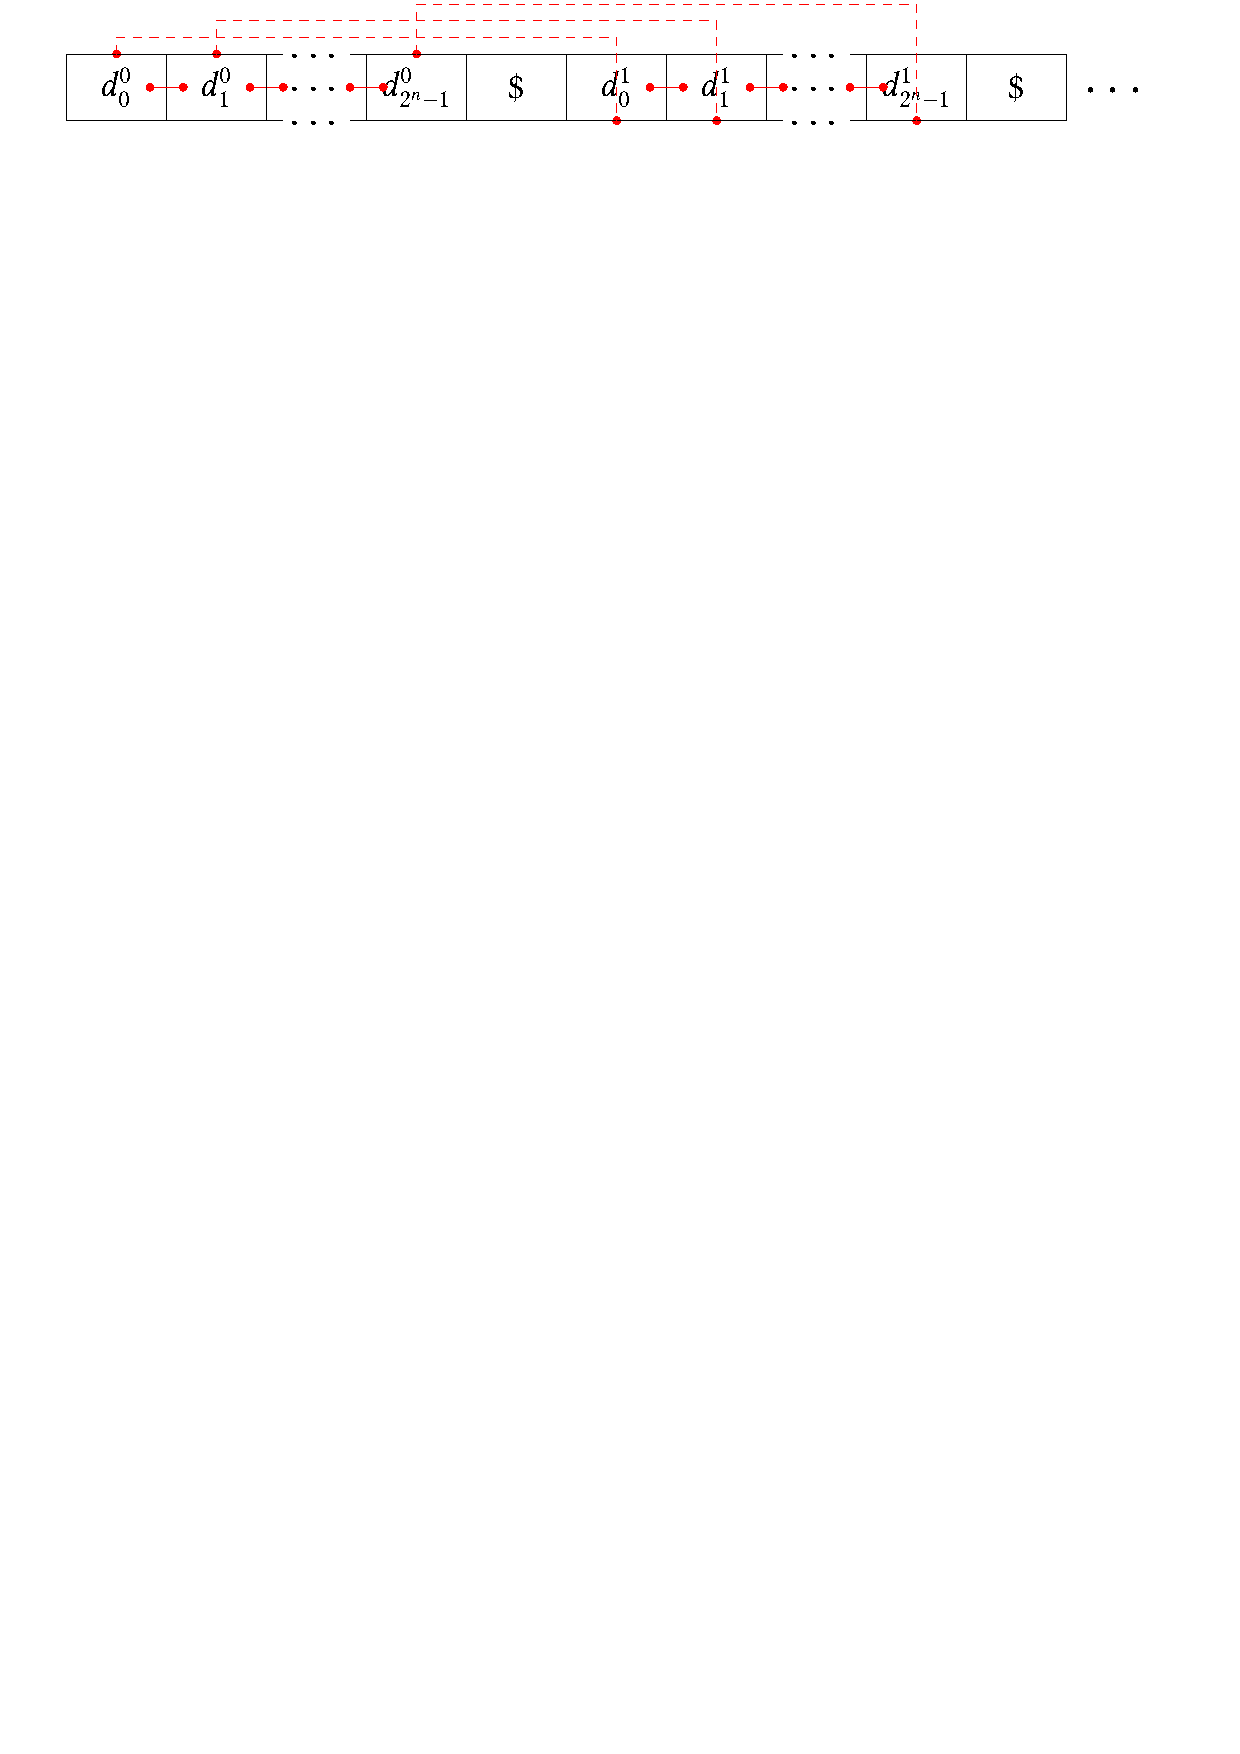
\includegraphics[scale=0.42]{Chaps/Timelines/row1.pdf}\hspace{1pt}
    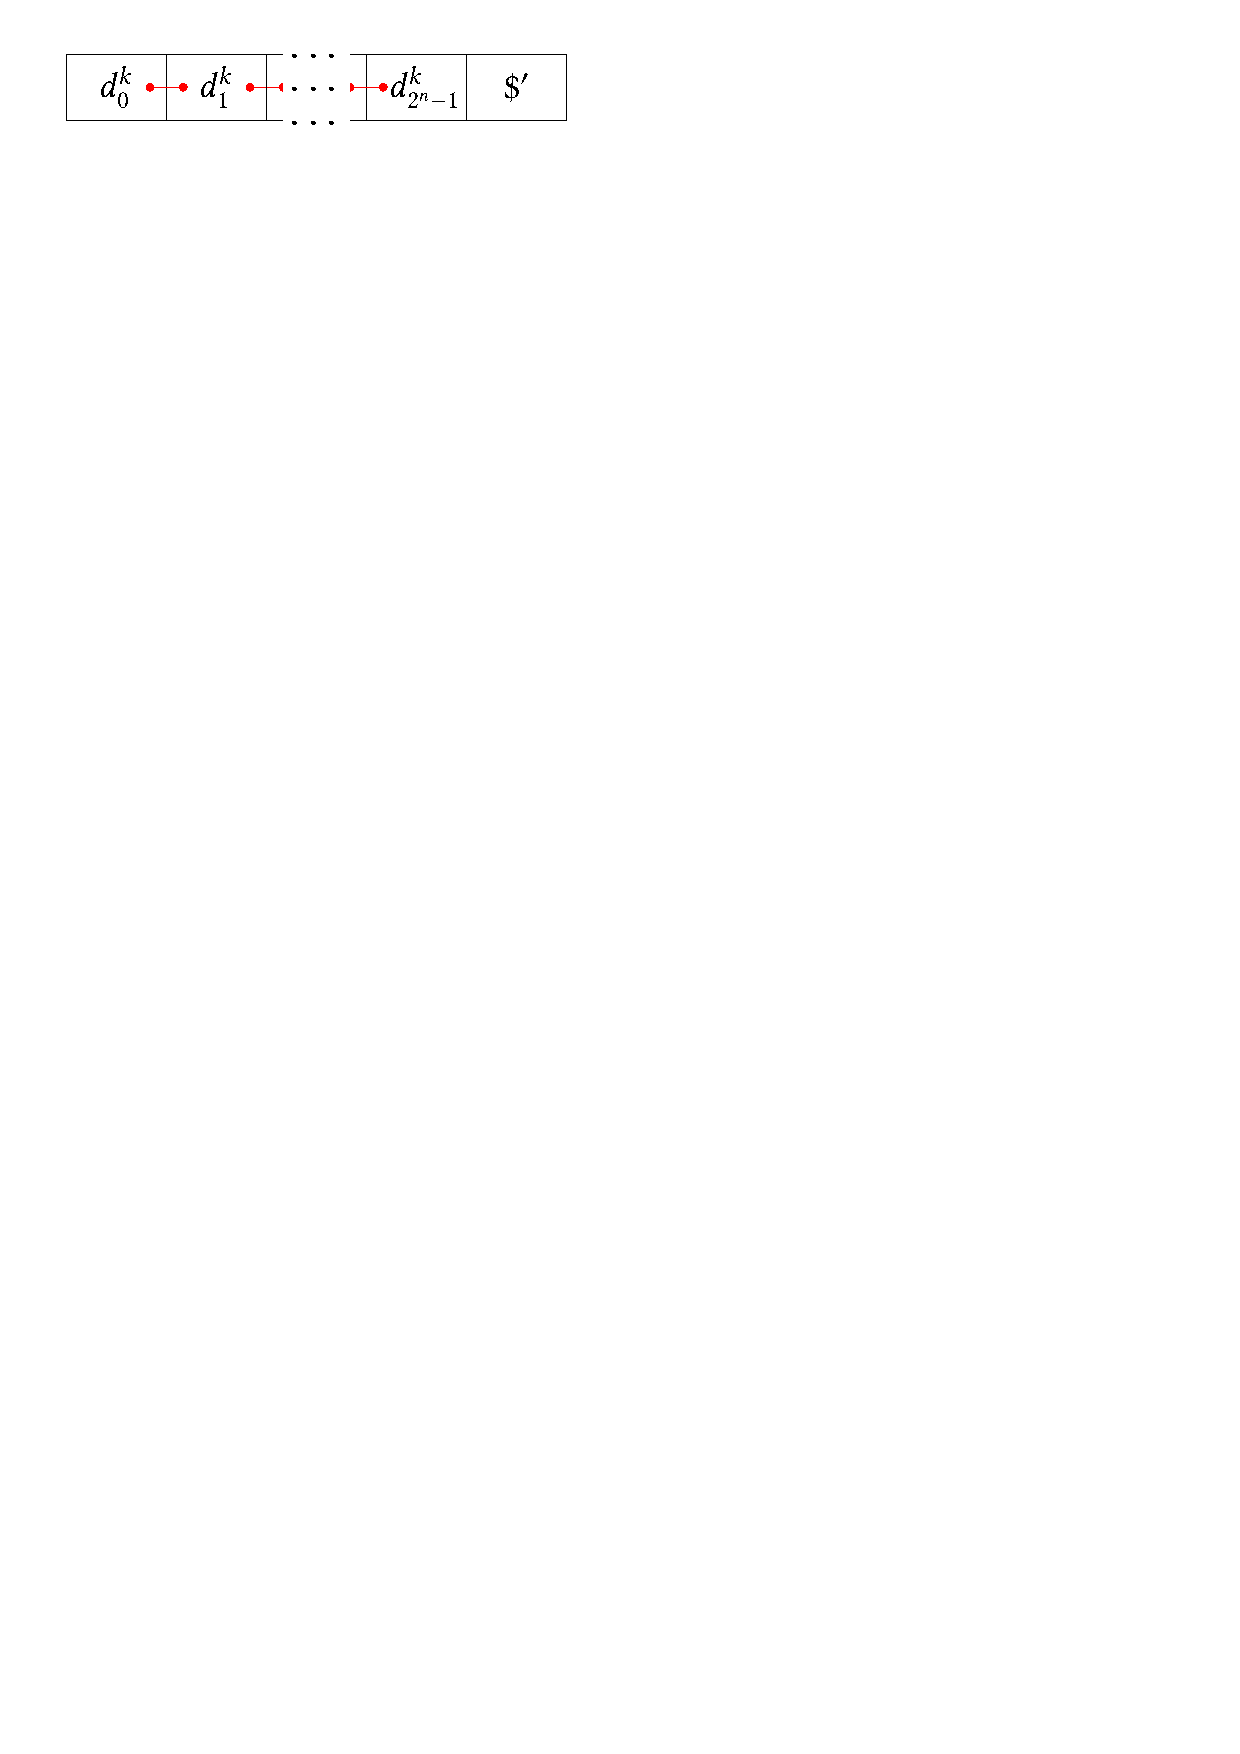
\includegraphics[scale=0.42]{Chaps/Timelines/row2.pdf}
%    \vspace{-0.4cm}
    \caption{A timeline encoding the ordered concatenation of the rows of a tiling. Red lines represent the horizontal and vertical constraints among domino-types.}\label{fig:rowEXPhardTP}
\end{figure}

We observe that $T$ guarantees the horizontal constraint among domino-types, and that it allows only occurrences of $\$'$ after the first $\$'$. 

We start with the next simple trigger rules, one for each $v\in V$: 
\[o[y=v]\to o\leq^{\mathsf{s},\mathsf{e}}_{[0,2]} o.\] 
These, paired with the constraint function $D$, enforce
all tokens' durations to be exactly 2. This is done for technical convenience: intuitively, since we exclude singular intervals, requiring, for instance, that a token $o'$ starts  $t$ instants of time after the end of $o$, with $t\in [\ell,\ell+1]$ and even $\ell\in\Nat$, boils down to $o'$ starting \emph{exactly} $\ell$ instants after the end of $o$. We also observe that, given the constant token duration, in this proof the density of the time domain does not play any role.

We now define the following synchronization rules (of which all trigger ones are simple and future). The next ones state (together) that the \emph{first occurrence} of (a token having value) $\$$ starts exactly at $2\cdot 2^n$:
\begin{equation}\label{equat:1}
    \true \to \exists o[y=\$]. o\geq^{\mathsf{s}}_{[0,1]} 2\cdot 2^n ,
\end{equation}
and 
\begin{equation}\label{eq:2}
    o[y=\$] \to  o\geq^{\mathsf{s}}_{[0,+\infty[} 2\cdot 2^n.
\end{equation}
Thus, all tokens before such a first occurrence of $\$$ have a value in $\Delta$.

Every occurrence of $\$$ must be followed, after exactly $2\cdot 2^n$ instants of time (namely, after $2^n$ tokens), by another occurrence of $\$$ or of $\$'$.
\begin{multline}\label{eq:3}
o[y=\$]\to \\ (\exists o'[y=\$]. o\leq ^{\mathsf{e},\mathsf{s}}_{[2\cdot 2^n,2\cdot 2^n+1]} o') \vee (\exists o''[y=\$']. o\leq ^{\mathsf{e},\mathsf{s}}_{[2\cdot 2^n,2\cdot 2^n+1]} o'').
\end{multline}

Now we force every token with value $d\in \Delta$ either $(i)$ to be followed, after $2\cdot 2^n$ instants, by another token with value  $d'\in\Delta$, in particular, satisfying the vertical requirement, i.e., $[d]_{\Up}=[d']_{\Down}$, or $(ii)$ to be in the last row (which is terminated by $\$'$). For each $d\in \Delta$, 
\begin{multline}\label{eq:4}
o[y=d]\to \\ \Big(\smashoperator{\bigvee_{d'\in\Delta, \,[d]_{\Up}=[d']_{\Down}}} \exists o'[y=d']. o\leq ^{\mathsf{e},\mathsf{s}}_{[2\cdot 2^n,2\cdot 2^n+1]} o'\Big) \vee (\exists o''[y=\$']. o\leq ^{\mathsf{e},\mathsf{s}}_{[0,2\cdot 2^n-2]} o'').
\end{multline}

It is straightforward to check that rules (\ref{equat:1}), (\ref{eq:2}), (\ref{eq:3}), and (\ref{eq:4}), along with the horizontal constraint guaranteed by the function $T$, enforce the following property.
\begin{proposition}
There exists $k'\in\Nat^+$ such that
all tokens with value $\$$ end at all and only times $k\cdot 2(2^n+1)$, for $1\leq k< k'$. Moreover the first token with value $\$'$ ends at time $k'\cdot 2(2^n+1)$. Finally, all other tokens having end time less than $k'\cdot 2(2^n+1)$ have value in $\Delta$ and satisfy the horizontal and vertical constraints.
\end{proposition}

Finally, we settle the initialization and acceptance requirements by means of the following pair of trigger-less rules:
\[
    \true \to \exists o[y=d_\Init]. o\geq^{\mathsf{s}}_{[0,1]} 0,
\]
\[
    \true \to \exists o[y=d_\Final]\exists o'[y=\$']. o\leq^{\mathsf{e},\mathsf{s}}_{[0,1]} o'.
\]
The former rule states that a token with value $d_\Init$ must start at $t=0$, the latter that a
token with value $d_\Final$ must occur just before the terminator of the last row $\$'$.


To conclude the proof, we observe that the state variable $y=(V,T,D)$ as well as all synchronization rules can be generated in polynomial time in the size of the instance $\Instance$ of the domino-tiling problem (in particular, note that all interval bounds and time constants of time-point atoms have a value, encoded in binary, which is in $O(2^n)$).
\end{proof}